\documentclass[twoside]{article}
\usepackage{float} 
\usepackage{bookmark}
\usepackage{titlesec}
\usepackage{titling}
\usepackage{graphicx}
\usepackage{tikz}
\usepackage{pgfplots}
\usepackage{caption}
\usepackage{multirow}
\usepackage{fancyhdr} 
\usepackage{graphicx}
\usepackage{hyperref}
\usepackage{titlesec}
\usepackage{natbib}
\usepackage{amsmath}
\usepackage{amsthm}
\usepackage{amssymb}
\usepackage{parskip}
\usepackage[utf8]{inputenc}
\usepackage{multicol}
\usepackage{csvsimple}
\usepackage{longtable}
\usepackage{textgreek}
\usepackage{listings}
\usepackage{booktabs}
\usepackage{longtable}


\title{\textbf{Malaria: Molecular Mechanisms and Therapeutic Targets}}
\author{Rahul Chavan}
\markboth{Malaria: Molecular Mechanisms and Therapeutic Targets}{\thepage}
\date{\today}

\pagestyle{fancy}
\fancyhf{}
\fancyhead[LO,RE]{\leftmark}
\fancyfoot[C]{\thepage}


\usepackage[left=1in, right=1in, top=1in, bottom=1in]{geometry}
\renewcommand{\maketitle}{
 \begin{center}
    
        
\includegraphics[width=2cm]{IISc_Master_Seal_Black.jpg}
        \vspace{0.5cm}

        \Large
        \textbf{\thetitle}
        
        \vspace{0.5cm}
        
        \Large
        \theauthor

        \small{Bachelor of Science (Research), Indian Institute of Science, \href{mailto:rahulchavan@iisc.ac.in}{rahulchavan@iisc.ac.in}}
        
        \vspace{0.2cm}
        
        \large
        \thedate

        \vspace{0.5cm}

        \markboth{Malaria: Molecular Mechanisms and Therapeutic Targets}{\thepage}

        \hrule  
        
    \end{center}
}

\pgfplotsset{compat=1.18}
\begin{document}
\maketitle

%In this assignment, you are required to do a brief analysis of the disease allotted to you (in my case it is malaria). 
%There will be two parts of the assignment.
 
%Part A: Provide a brief overview of the disease. Describe the cause and effect of the perturbation involved. 
%Provide the details of the organ, tissues and cells of the human body affected, the molecular map of the disease process, 
%and the proteins/genes playing a role.
 

%Part B: Once you get the overall molecular basis of the disease, list down the proteins and 
%their corresponding RefSeq IDs which are commonly used drug targets. 
%Also mention if there is any other protein which you think can be used as a therapeutic target.

\begin{abstract}
    Malaria is a life-threatening disease caused by plasmodium parasites that are transmitted to people through the
    bites of infected female anopheles mosquitoes. It is a major public health problem in many parts of the world.
    This report provides an overview of the molecular mechanisms of malaria pathogenesis and the proteins that can be targeted for the development of antimalarial drugs.
    The report is divided into two parts. Part A provides a brief overview of malaria, including the cause and effect of the perturbation involved, the organs, tissues, and cells affected, and the proteins playing a role in the disease process. Part B lists the proteins and their corresponding RefSeq IDs which can be used as therapeutic targets for the treatment of malaria. 
    The report is based on the current understanding of the molecular mechanisms of malaria pathogenesis and the proteins that can be targeted for the development of antimalarial drugs. 

    \textbf{Keywords:} Malaria, Plasmodium, Antimalarial Drugs, Therapeutic Targets, RefSeq IDs


\end{abstract}

\section*{Part A: Overview of Malaria}

    Six plasmodial species present a significant health threat for humans; Plasmodium falciparum 
    is usually considered the most important in terms of deaths. P. vivax is a major cause of illness across large parts of the world, and it is increasingly argued 
    that deaths, due to this parasite, have been underestimated. P. ovale curtisi, P. ovale wallikeri, and 
    P. malariae are much less common causes of significant disease. Recently the simian parasite P. knowlesi has emerged as a local but 
    important cause of disease (including severe disease) in Malaysia and other areas of southeast Asia, where it is predominantly a zoonosis, 
    with no definite evidence of primary human-to-human transmission.

    \begin{figure}[H]
        \centering
        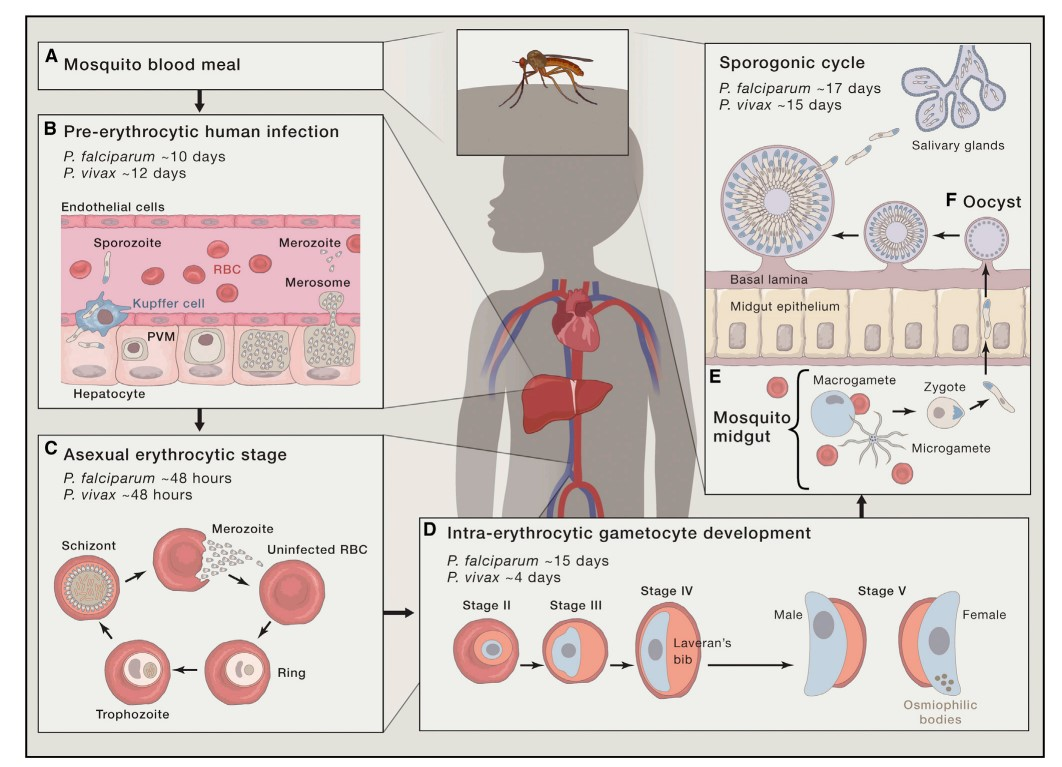
\includegraphics[width=0.8\textwidth]{malarialifecycle.jpg}
        \caption{Malaria Life Cycle}
        \label{fig: Malaria Life Cycle}
    \end{figure}


\begin{multicols}{2}

    \subsection*{Cause and Effect of the Perturbation}
    Sporozoites are the infectious form of plasmodium that enter human host on the bite of female anopheles mosquito. 
    They reach the hepatocytes via the blood stream and multiply inside them to form the merozoites (pre erythrocytic schizogony). 
    This corresponds to incubation period during which the peripheral blood is sterile, the patient is asymptomatic and non-infectious. 
    The hepatocytes rupture to release merozoites into blood stream wherein they enter the RBCs to carry out the erythrocytic schizogony. 
    A few re-enter the hepatocytes (only in case of P. vivax and P. ovale) to carry out the exo erythrocytic schizogony or stay dormant for 
    several years to cause a relapse of malaria later. During erthrocytic schizogony within RBCs, a single merozoite transforms into early trophozoite (ring form) 
    followed by late trophozite and then undergoes several mitotic divisions to form the schizont. This corresponds to period of prodromal symptoms. 
    The schizont transforms into several merozoites which are released upon the rupture of the RBC and lead to the malarial paroxysm of fever with chills and rigors. 
    These merozoites then enter other RBCs. A few transform into male and female gametocytes. When female anopheles sucks the blood of such infected human, 
    it ingests these gametocytes which undergo sexual cycle within the mosquito to form sporozoites, thus completing the plasmodium life cycle. 
    
    
    
    \subsection*{Organs, Tissues, and Cells Affected, and Proteins playing a role}

    \subsubsection*{Liver}
    After injection into the dermis, the protein Trap-like protein (TLP) plays a role in
    exit from the dermis, as mutant sporozoites lacking its function
    display normal gliding motility but cannot enter the circulation.
    The sporozoites then enter the blood stream and are transported to the liver by a process called traversal.
    Proteins required for traversal are SPECT (sporozoite microneme protein
    essential for traversal), SPECT2 (also known as perforin-like protein 1, PLP1), CelTOS (cell traversal protein for ookinetes and sporozoites),
    phospholipase (PL), and gamete egress
    and sporozoite traversal protein (GEST). The function of these
    proteins in cell traversal is not understood, although SPECT2
    has a membrane attack complex/perforin-like (MAC/PF) domain,
    suggesting that it plays a role in punching holes in membranes.
    The sporozoites then enter the liver sinusoids and traverse the
    endothelial cells to reach the hepatocytes. Sporozoites injected
    into the dermis are in "migratory mode" and upon interaction
    with hepatocytes convert to "invasive mode".
    This switch is due to the recognition  hepatocytes through binding
    higher sulfated forms of heparin sulfate proteoglycans (HSPGs)
    activating calcium-dependent protein kinase 6 (CDPK6). The tetraspanin CD81 and scavenger receptor
    B1 (SR-B1) are human hepatocyte surface proteins required
    for invasion and formation of a parasitophorous vacuole by
    P. falciparum sporozoites. Proteins such as the circumsporozoite protein (CSP), thrombospondin-related
    adhesive protein (TRAP) and apical membrane antigen 1 (AMA1)
    are involved in the invasion of hepatocytes by sporozoites. The sporozoites then
    transform into liver stages (also known as exoerythrocytic
    forms) and replicate within the hepatocytes. 
%Pre-invasion involves robust interaction between the mero zoite and erythrocyte resulting in parasite actomyosin motor driven deformation of the host cell (Weiss et al., 2015) 
%(Figure 2). This step involves two ligand families of type 1 membrane pro teins in P. falciparum, 
%the erythrocyte binding-like proteins (EBLs) and P. falciparum reticulocyte-binding protein homologs (PfRhs). These protein ligands bind specific receptors including glycophorin A, B, C and complement receptor 1 (CR1). Although the functions of individual members of these families display redundancy, their overall function is essential in P. falciparum (re viewed in Tham et al., 2012). PfRh and EBL proteins also play a role in signaling activation of subsequent steps in invasion. Exposure of P. falciparum merozoites to low-potassium ion con centrations in blood plasma, after egress from the host cell, leads to a rise in cytosolic calcium levels through a phospholi pase C-mediated pathway, triggering release of EBA-175, an EBL family member (Singh et al., 2010). Binding of EBA-175 to its receptor, glycophorin A, triggers release of proteins from the rhoptries. This work provides evidence of the importance of these protein families in sensing and binding to erythrocytes but also signaling downstream invasion events. Similarly, PfRh1 is linked to Ca2+ signaling in the merozoite (Gao et al., 2013), and phosphorylation of the cytoplasmic tail of PfRh4 by the P. falciparum casein kinase 2 (PfCK2) is required for invasion through the PfRh4-CR1 parasite-host interaction (Tham et al., 2015). Calcineurin is also involved in attachment of merozoites, perhaps through stabilizing the dimerization of EBL and PfRh proteins, as this is critical for host-receptor ligation and signal transduction for subsequent events in invasion
   
    \subsubsection*{Red Blood Cells}
    The merozoites are released from the liver and enter the blood stream, where they invade red blood cells (RBCs) and replicate
    within them. The invasion of RBCs by merozoites is a complex process that involves the interaction of parasite proteins with
    RBC surface receptors. Proteins such as the merozoite surface protein 1 (MSP1) and the apical membrane antigen 1 (AMA1) are
    involved in the invasion of RBCs by merozoites. Once inside the RBCs, the parasite replicates and undergoes several rounds of
    asexual replication, leading to the release of merozoites and the destruction of RBCs. This process is responsible for the
    clinical symptoms of malaria, including fever, chills, and anemia. The sequestration of infected RBCs in the microvasculature
    is a key feature of severe malaria and is mediated by parasite proteins such as the erythrocyte membrane protein 1 (PfEMP1)
    and the reticulocyte binding protein homolog 5 (RH5).
    The sequestration of infected RBCs is also thought to play a role in the modulation of host immune responses and the development of severe
    complications such as cerebral malaria and multi-organ failure. 
%The AQP4 channels facilitate the flux of ISF into perivascular spaces to be mixed with CSF87,88, and this eventually contributes to the clearance of particles from the CSF. 
%Interestingly, dilatation at perivascular spaces and astroglia and reduced expression of AQP4 protein have been reported during cerebral malaria in animal models

    \subsubsection*{Brain}
    Cerebral malaria is a severe complication of malaria that is characterized by the sequestration of infected RBCs in the brain microvasculature.
    This leads to the disruption of the blood-brain barrier and the development of neurological symptoms such as coma, seizures, and
    cognitive impairment. The sequestration of infected RBCs in the brain is mediated by parasite proteins such as the erythrocyte membrane protein 1 (PfEMP1)
    and the reticulocyte binding protein homolog 5 (RH5).
    The AQP4 channels facilitate the flux of ISF into perivascular spaces to be mixed with CSF, 
    and this eventually contributes to the clearance of particles from the CSF.
    Interestingly, dilatation at perivascular spaces and astroglia and reduced expression of AQP4 protein have been reported during cerebral malaria.
   
    \subsubsection*{Other Organs}
    Malaria can also affect other organs such as the lungs, kidneys, and liver, leading to complications such as acute respiratory distress syndrome,
    acute kidney injury, and hepatic dysfunction. The sequestration of infected RBCs in the microvasculature of these organs is thought to play a role in the development of these complications.
    The parasite proteins involved in the sequestration of infected RBCs in these organs are not well characterized, but it is likely that they are similar to those involved in the sequestration of infected RBCs in the brain.


\end{multicols}

\begin{figure}[H]
    \centering
    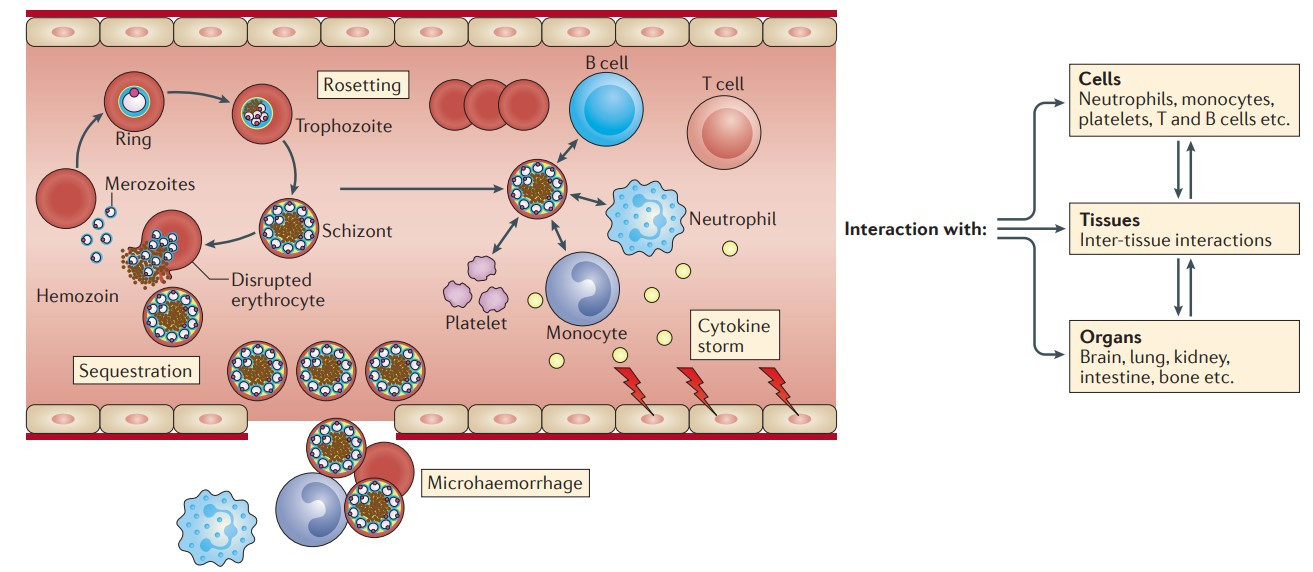
\includegraphics[width=0.8\textwidth]{bloodstream.jpg}
    \caption{Outcomes of Plasmodium infection of red blood cells in the bloodstream}
    \label{fig: Outcomes of Plasmodium infection of red blood cells in the bloodstream}
\end{figure}


\begin{figure}[H]
    \centering
    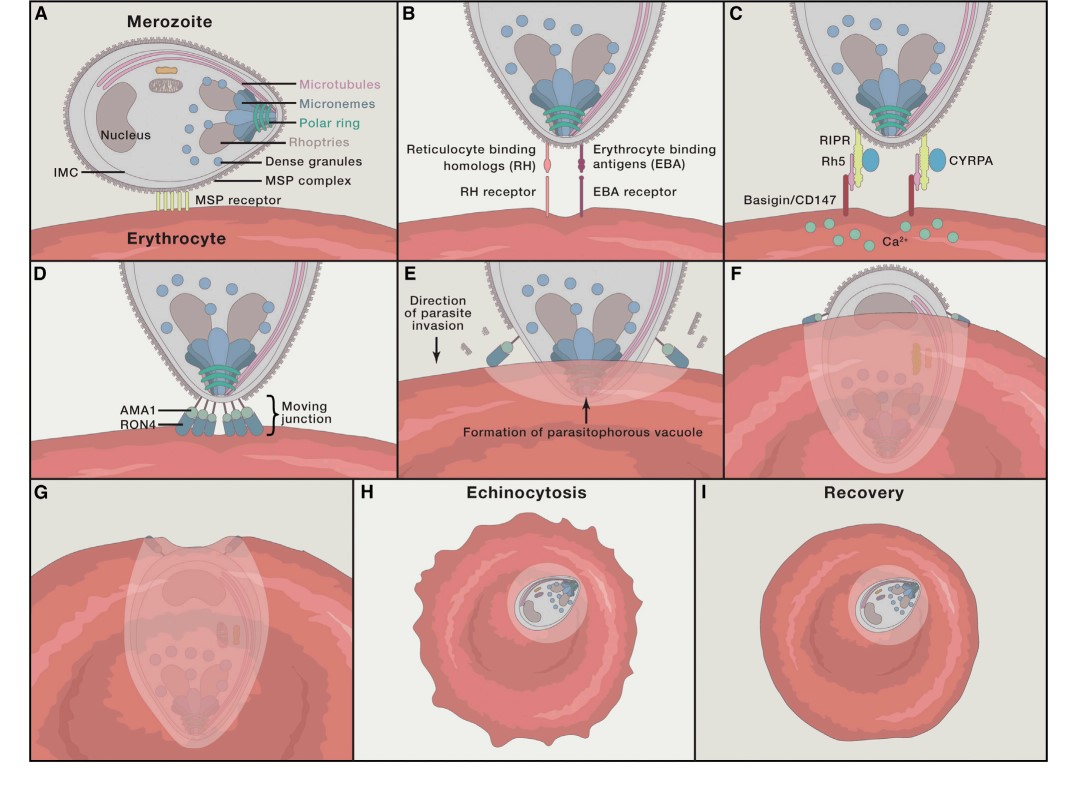
\includegraphics[width=0.8\textwidth]{erythrocytemolmap.jpg}
    \caption{Malaria Pathogenesis in Red Blood Cells}
    \label{fig: Malaria Pathogenesis in Red Blood Cells}
\end{figure}


\section*{Part B: Therapeutic Targets}

\begin{multicols}{2}

    Treatment of malaria aims at completely curing the patient,
    preventing progression to severe disease, preventing malaria
    relapse (due to survival of exo erythrocytic forms in hepatocytes in P. vivax and P. ovale) and recrudescence 
    (due to persistence of erythrocytic forms in P. falciparum), interrupting
    the transmission of malaria and preventing drug resistance.

    The following are the types of drugs used for the treatment of malaria:
    \begin{itemize}
        \item Clinical curative: Drugs that treat the clinical attack of
        malaria by eliminating the erthrocytic stage of
        plasmodium
        \item High efficacy drugs: Artemisinin derivatives, chloroquine, amodiaquine, mefloquine, quinine, lumifantrine
        \item Low efficacy drugs: Doxycycline, clindamycin, sulphonamides, pyrimethmine
        \item Radical curative: Drugs that remove the exo erythrocytic stage of plasmodium in the hepatocytes. 
        Not needed in P. falciparum. E.g., Primaquine
        \item Transmission blocking: Drugs that prevent the transmission of malaria from human to mosquito. E.g., Primaquine
        \item Gametocidal: These drugs kill the plasmodial gametocytes, thus breaking the transmission chain. E.g.,
              Primaquine is gametocidal to all plasmodia species, 8-amodiaquins
    \end{itemize}
            
    
\end{multicols}

\subsection*{Commonly Used Drug Targets}

The following are the approaches that have
been successful, and the ones which are in preclinical and clinical development. Potential targets are listed which have had in vivo and 
in vitro validation, and are being pursued for drug discovery.

\begin{figure}[H]
    \centering
    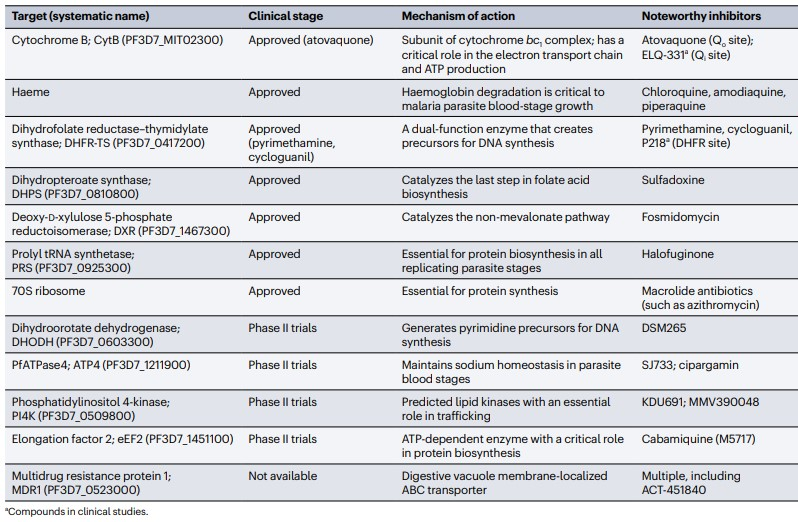
\includegraphics[width=0.8\textwidth]{drugtargets1.jpg}
    \caption{Antimalarial Drug Targets with Clinical Validation} 
    \label{fig: Antimalarial Drug Targets with Clinical Validation}
\end{figure}

\begin{figure}[H]
    \centering
    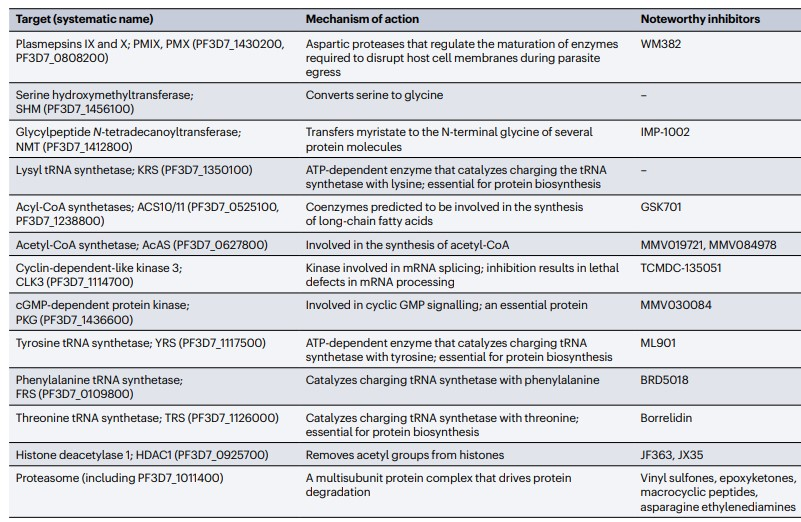
\includegraphics[width=0.8\textwidth]{drugtargets2.jpg}
    \caption{Antimalarial Drug Targets with in Vivo Validation}
    \label{fig: Antimalarial Drug Targets with in Vivo Validation}
\end{figure}

\begin{figure}[H]
    \centering
    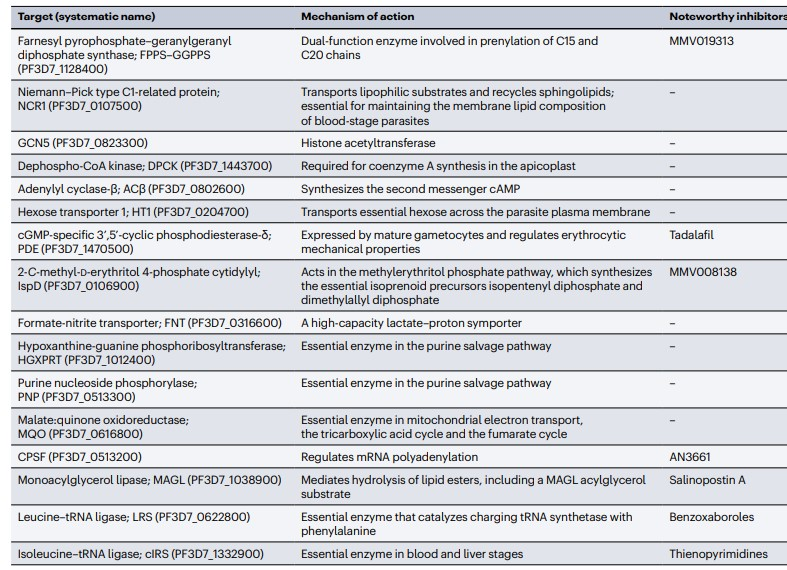
\includegraphics[width=0.8\textwidth]{drugtargets3.jpg}
    \caption{Antimalarial Drug Targets with in Vitro Validation}
    \label{fig: Antimalarial Drug Targets with in Vitro Validation}
\end{figure}

The following table lists the proteins and their corresponding RefSeq IDs which can be used as therapeutic targets for the treatment of malaria.
This information is based on the literature review and the current understanding of the molecular mechanisms of malaria pathogenesis.


%1.	Merozoite surface protein 1 (MSP1): NP_702759.1
%2.	Apical membrane antigen 1 (AMA1): NP_705275.1
%3.	Erythrocyte membrane protein 1 (PfEMP1): NP_703470.1
%4.	Reticulocyte binding protein homolog 5 (RH5): NP_703586.1
%5.	Spectrin: NP_001239243.1
%6.	Ankyrin: NP_705292.1
%7.	Band 3: NP_705586.1
%8.	Glycophorin A: NP_002087.1
%9.	Complement receptor 1 (CR1): NP_000642.2
%10.	Thrombospondin-related adhesive protein (TRAP): NP_705455.1
%11.	Apical membrane antigen 1 (AMA1): NP_705275.1
%Trap-like protein (TLP): RefSeq ID - NP_701225.1
%Sporozoite Microneme Protein Essential for Traversal (SPECT): RefSeq ID - NP_703996.1
%Perforin-like Protein 1 (PLP1, also known as SPECT2): RefSeq ID - NP_705539.1
%Cell Traversal Protein for Ookinetes and Sporozoites (CelTOS): RefSeq ID - NP_705465.1
%Phospholipase (PL): RefSeq ID - NP_703359.1 (assuming this refers to a Plasmodium phospholipase)
%Gamete Egress and Sporozoite Traversal Protein (GEST): RefSeq ID - NP_703801.1
%Calcium-Dependent Protein Kinase 6 (CDPK6): RefSeq ID - NP_703961.1 (assuming this refers to Plasmodium CDPK6)
%CD81: RefSeq ID - NP_004342.1 (human CD81)
%Scavenger Receptor B1 (SR-B1): RefSeq ID - NP_005625.2 (human SR-B1)
%Circumsporozoite Protein (CSP): RefSeq ID - NP_703391.1
%Thrombospondin-related Adhesive Protein (TRAP): RefSeq ID - NP_705455.1
%Apical Membrane Antigen 1 (AMA1): RefSeq ID - NP_033828.1


\begin{longtable}{|c|c|}
    \hline
    \textbf{Protein} & \textbf{RefSeq ID} \\
    \hline
    Merozoite surface protein 1 (MSP1) & NP\_702759.1 \\
    Apical membrane antigen 1 (AMA1) & NP\_705275.1 \\
    Erythrocyte membrane protein 1 (PfEMP1) & NP\_703470.1 \\
    Reticulocyte binding protein homolog 5 (RH5) & NP\_703586.1 \\
    Spectrin & NP\_001239243.1 \\
    Ankyrin & NP\_705292.1 \\
    Band 3 & NP\_705586.1 \\
    Glycophorin A & NP\_002087.1 \\
    Complement receptor 1 (CR1) & NP\_000642.2 \\
    Trap-like protein (TLP) & NP\_701225.1 \\
    Sporozoite Microneme Protein Essential for Traversal (SPECT) & NP\_703996.1 \\
    Perforin-like Protein 1 (PLP1, also known as SPECT2) & NP\_705539.1 \\
    Cell Traversal Protein for Ookinetes and Sporozoites (CelTOS) & NP\_705465.1 \\
    Phospholipase (PL) & NP\_703359.1 \\
    Gamete Egress and Sporozoite Traversal Protein (GEST) & NP\_703801.1 \\
    Calcium-Dependent Protein Kinase 6 (CDPK6) & NP\_703961.1 \\
    CD81 & NP\_004342.1 \\
    Scavenger Receptor B1 (SR-B1) & NP\_005625.2 \\
    Circumsporozoite Protein (CSP) & NP\_703391.1 \\
    Thrombospondin-related Adhesive Protein (TRAP) & NP\_705455.1 \\
    \hline
    \caption{Proteins and their corresponding RefSeq IDs}
\end{longtable}


\section*{References}
\begin{enumerate}
    \item Milner DA Jr. Malaria Pathogenesis. Cold Spring Harb Perspect Med. 2018 Jan 2;8(1):a025569. doi: 10.1101/cshperspect.a025569. PMID: 28533315; PMCID: PMC5749143.
    \item Cowman AF, Healer J, Marapana D, Marsh K. Malaria: Biology and Disease. Cell. 2016 Apr 7;167(3):610-24. doi: 10.1016/j.cell.2016.07.055. PMID: 27716510.
    \item Gamo FJ, Sanz LM, Vidal J, de Cozar C, Alvarez E, Lavandera JL, Vanderwall DE, Green DV, Kumar V, Hasan S, Brown JR, Peishoff CE, Cardon LR, Garcia-Bustos JF. Thousands of chemical starting points for antimalarial lead identification. Nature. 2010 Jul 29;465(7296):305-10. doi: 10.1038/nature09107. PMID: 20485426.
    \item World Health Organization. Guidelines for the treatment of malaria. 3rd ed. Geneva: World Health Organization; 2015.
    \item World Health Organization. World Malaria Report 2020. Geneva: World Health Organization; 2020.
    \item Coban C, Lee MSJ, Ishii KJ. Tissue-specific immunopathology during malaria infection. Nat Rev Immunol. 2018 Apr;18(4):266-278. doi: 10.1038/nri.2017.138. Epub 2018 Jan 15. PMID: 29332936; PMCID: PMC7097228.
    \item Basu S, Sahi PK. Malaria: An Update. Indian J Pediatr. 2017 Jul;84(7):521-528. doi: 10.1007/s12098-017-2332-2. Epub 2017 Mar 30. PMID: 28357581. 
    \item Siqueira-Neto, J.L., Wicht, K.J., Chibale, K. et al. Antimalarial drug discovery: progress and approaches. Nat Rev Drug Discov 22, 807-826 (2023). 
\end{enumerate}




\end{document}
